% This is samplepaper.tex, a sample chapter demonstrating the
% LLNCS macro package for Springer Computer Science proceedings;
% Version 2.20 of 2017/10/04
%
\documentclass[runningheads]{llncs}
%
%\usepackage{fullpage}
%\usepackage{setspace}
%\onehalfspacing
\usepackage{listings}
\usepackage{graphicx}
% Used for displaying a sample figure. If possible, figure files should
% be included in EPS format.
\usepackage{makecell}
\renewcommand\theadfont{\bfseries}
%
% If you use the hyperref package, please uncomment the following line
% to display URLs in blue roman font according to Springer's eBook style:
% \renewcommand\UrlFont{\color{blue}\rmfamily}

\begin{document}
%
\title{BLAST: Block Applications for Things}
%
%\titlerunning{Abbreviated paper title}
% If the paper title is too long for the running head, you can set
% an abbreviated paper title here
%
\author{Michael Freund\inst{1}\orcidID{0000-0003-1601-9331} \and
Thomas Wehr\inst{1}\orcidID{0000-0002-0678-5019} \and
Andreas Harth\inst{1,2}\orcidID{0000-0002-0702-510X}}
%
\authorrunning{M. Freund et al.}
% First names are abbreviated in the running head.
% If there are more than two authors, 'et al.' is used.
%
\institute{Fraunhofer Institute for Integrated Circuits IIS, Nürnberg, Germany 
\email{firstname.lastname@iis.fraunhofer.de}\\
\and
Friedrich–Alexander University Erlangen-Nürnberg, Nürnberg, Germany}
%
\maketitle              % typeset the header of the contribution
%
\begin{abstract}
  An open research challenge in the deployment of digital twins is the interaction with humans.
  To facilitate this, we have created a digital twin based on Web of Things technology and a block-based visual programming language and execution environment called BLAST.
  We show that BLAST can be used to create programs that interact with a digital twin and IoT devices to control and monitor a process.

\keywords{Block-based Programming \and Web of Things.}
\end{abstract}
%
%
%
\setcounter{footnote}{0}
\section{Introduction}
IoT devices can be used for state monitoring, energy consumption analysis, simulation and intelligent optimization \cite{CIMINO2019103130}.
However, there are still some research challenges that need to be overcome.
According to Semeraro et al. \cite{SEMERARO2021103469}, the main research challenges in implementing a DT are in the areas of architecture, interoperability, and  interaction capabilities.

Architecture refers to the fact that no design standard currently exists, so different DTs use varying technologies, interfaces, and communication protocols.
A reference architecture could contribute to the flexibility and reusability of DTs.
Interoperability includes a DT's ability to capture a multi-stage product lifecycle, which requires collecting data from external sources and from other companies.
However, to achieve this, data exchange between multiple DTs must be enabled.
The area of interaction capabilities refers to the fact that Digital Twins will not be involved in any important decisions without humans. Therefore, humans should find it easy to interact with DTs. 
Some other authors have also suggested that human-computer interaction is an open research question that needs to be resolved before widespread deployment of DTs in industry \cite{KUEHNER20211227}.

In this paper, we want to address the problem of human-digital twin interaction.
Semeraro et al. \cite{SEMERARO2021103469} propose in this context to focus on the development of the Digital Twin so that it is able to interact smoothly with humans.
Our proposed solution follows this approach.
We have described a digital twin using RDF and ontologies in human and machine-readable form.
However, our solution includes another perspective to improve human-DT interaction.
We developed an easy-to-use interaction interface for humans with digital twins based on Google's Blockly\footnote{\url{https://developers.google.com/blockly/}}.
To show the feasibility of this approach, we developed and implemented a demonstrator for a commissioning process as a proof of concept.

\section{Block-based Visual Programming}
The programming languages currently in use are primarily text-based and are difficult to access for laypersons without prior knowledge.
One possible approach to improve accessibility and simplify the creation of computer programs is so-called Visual Programming (VP).
% Falls Platz dafür ist, die Definition für VP fand ich besser:
VP as defined by Myers \cite{myers1990taxonomies} refers to any system that allows the user to specify a program in a two (or more) dimensional fashion. Conventional textual languages are not considered two dimensional since the compiler or interpreter processes it as a long, one-dimensional stream. For a more in-depth definition of VP, the reader is referred to \cite{burnett1995visual}. 
VP does not require the user to enter any text, it is instead based on graphical elements like blocks, graphs, tables or diagrams.
Programs are created by arranging the available graphical elements in the correct order.
The block-based approach of VP has become established in recent years, especially as an entry point for novice programmers 
% Vorschläge für Referenzen
\cite{moors2018transitioning} \cite{weintrop2017blocks} \cite{chao2016exploring} \cite{HUNDHAUSEN200722} \cite{10.1145/2787622.2787712}.

Bau et al. \cite{1011453015455} pointed out that block-based programming languages teach programming concepts in a simple way due to an intuitive and friendly user interface and that after using block-based languages it is much easier for users to switch to traditional text-based languages.

The basic idea of the block-based approach is that predefined blocks with images or text are arranged into programs by using the drag-and-drop principle.
Blocks can be geometrically aligned with other compatible blocks, like in a jigsaw puzzle, to form complex programs.
Since blocks can only be arranged in the correct way, no syntax errors can occur \cite{10.11453341221} \cite{maloney2010scratch} \cite{10.1145/1089733.1089734} \cite{lye2014review}.
The created block programs can be translated into any predefined programming language, resulting in a normal source code. 
The block-based approach can be used not only for learning programming concepts, but also for more complex problems.
For example, it has been shown that block languages can be successfully used in programming industrial robots \cite{8120406} \cite{ghazal2016framework} \cite{tomlein2017visual} or executing SPARQL queries \cite{7369012}. Both areas, which normally require advanced programming skills. Furthermore, Ray examined the use of block-based programming languages for IoT devices in \cite{ray2017survey} and concluded that IoT seems to be suitably getting empowered by smooth entanglement and promotion with promising reduction in physical-digital interface. %Das ist ein direktes Zitat, muss man das anders schreiben?

\section{BLAST - Block Applications For Things}
Due to the success of block-based languages in different challenging areas, we have developed our own block language based on Google's Blockly\footnote{https://developers.google.com/blockly/} library. %Momentan zweimal die gleiche Fußnote auf einer Seite.
Blockly is a pure JavaScript library for creating block-based languages and editors.
Our block-based language simplifies the interaction with IoT devices, digital twins or other web resources without the need for a deeper understanding of different programming languages or network protocols such as Bluetooth or HTTP.
We have named our block language ''Block Applications For Things'', or BLAST for short (See figure \ref{fig1}).
The browser-based BLAST uses web Bluetooth to communicate with IoT devices, custom control and command blocks, and generates JavaScript code that can be used by any JavaScript interpreter.
To interact with the IoT devices, BLAST requires custom drivers for each device, which represent an extended form of the WoT TD % Beides noch nicht definiert
 and contain the metadata and interaction affordances as well as the JavaScript code needed for communication.

\begin{figure}
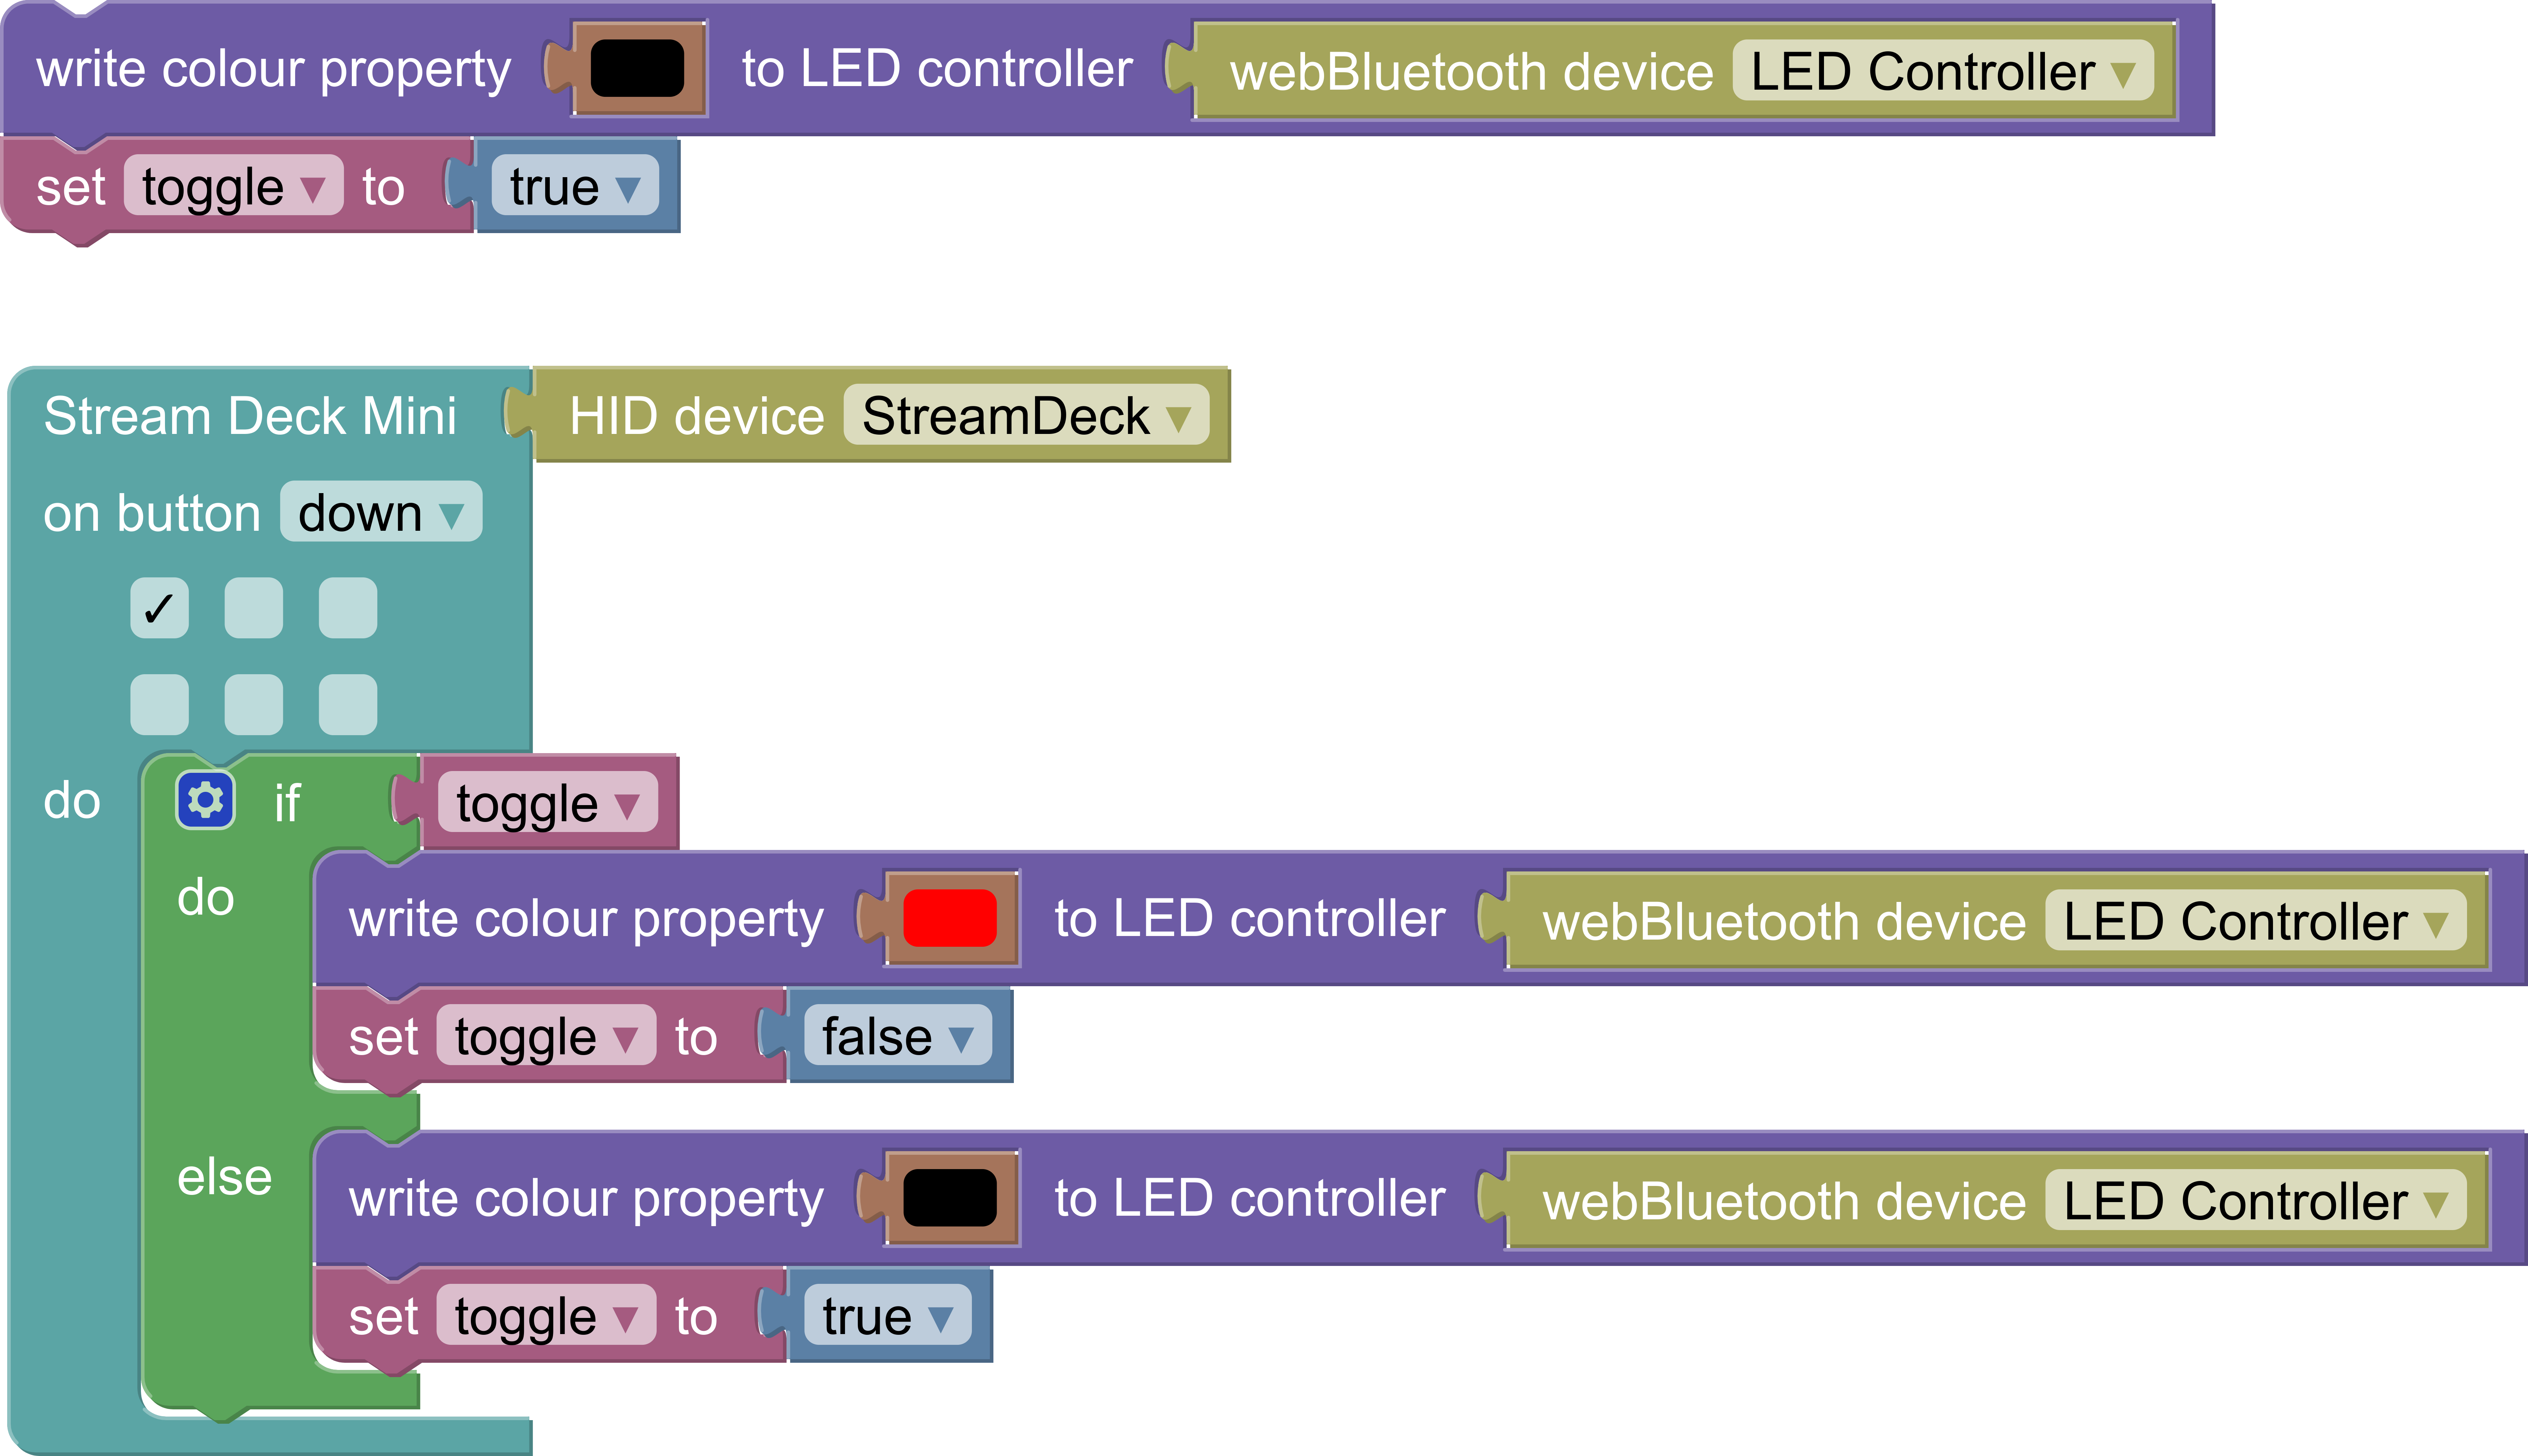
\includegraphics[width=\textwidth]{screenshot.png}%im Ordner sind noch 2 alternative Screenshots
\caption{Example BLAST program} \label{fig1}
\end{figure}

When choosing the vocabulary for our block-based language BLAST, we resorted to a mixture of natural language and computer language \cite{8120404}.
This means that in BLAST, the blocks are arranged into readable sentences, as in a natural language, but the blocks also contain a few technical programming terms, such as ''repeat while true'' instead of ''forever''.
This makes the BLAST vocabulary both understandable for beginners, but still flexible. Take the program in Figure \ref{fig1} as an example. One should easily figure out that it is used to toggle a Bluetooth LED light. Every time the user pushes the top-left button on their StreamDeck down, the LED light is toggled between red and off.

BLAST includes standards from other programming languages such as loops, functions, and variables, but also WoT and IoT related blocks that can be grouped under the three interaction affordances Properties, Actions, and Events.
Properties of connected IoT devices can be read and written, actions refer to long-running processes that can be initiated and events are asynchronous and based on the ''Event Conditon Action'' (ECA) rule.
If an event occurs, the condition is checked and if necessary the corresponding action is executed.
Furthermore, it is possible to send HTTP requests with arbitrary header and body or load knowledge graphs from a URI and execute SPARQL queries on the records, which allows interaction with read-write linked data APIs or other REST APIs.
If the available blocks are not sufficient to implement a desired functionality, there is a block in which native JavaScript code can be entered.
This block makes almost everything that is possible in JavaScript also possible in BLAST.

The currently best known tool for programming IoT devices using VP is Node-Red\footnote{https://nodered.org/}. Other than BLAST, Node-Red employs a flow-based programming paradigm, and therefore displays applications as graphs. The nodes in these graphs are black box processes, created by the developers, that can be connected to each other by the end user. The block-based approach utilized by BLAST provides more flexibility as its blocks are a lot more fine grained. Also, Node-Red does not implement the WoT standard, which hinders re-usability of code with applications other than Node-Red. Another application similiar to BLAST is Punya\cite{patton2021punya} an Android App development Application based on the MIT App Inventor\footnote{https://appinventor.mit.edu/}. Like Blast, Punya offers a block-based programming environment able to run SPARQL queries and utilizes services like sending a tweet. But Punya focuses on creating applications for Android devices only and solely communicates with the device's internal hardware. Other than BLAST, Punya apps are capable of working as a LDP-CoAP client to publish and access data on CoAP servers.

\section{Supported Devices and Services}

To demonstrate how BLAST can interact with WoT devices, we provide a Web of Things abstraction for devices communicating with Bluetooth Low Energy and USB Human Interface Devices (HID).
We also provide access to online APIs related to speech input and output and services like playing audio from a URI or invoking SPARQL queries on an online ressource.

\begin{center}
  \begin{tabular}{|c|c|c|}
  \hline
  \thead{Device} & \thead{Communication} & \thead{WoT interactions} \\
  \hline
  Eddystone Devices & BLE GATT & read/write Eddystone properties \\
  \hline
  HuskyLens\footnote{https://wiki.dfrobot.com/HUSKYLENS\_V1.0\_SKU\_SEN0305\_SEN0336} & BLE GATT & read sensor properties, invoke forget action \\
  \hline
  RGB LED Controller\footnote{https://aliexpress.com/item/4000208329326.html} & BLE GATT & write color properties \\
  \hline
  RuuviTag\footnote{https://ruuvi.com/ruuvitag/} & BLE GAP & \makecell{read sensor properties, read battery property, \\
  read/write txPower property, \\
  read movement counter propert,y \\
  read measurement sequence counter property} \\
  \hline
  StreamDeck\footnote{https://www.streamdeck.com/} & USB HID & \makecell{write display properties, \\ subscribe to button push events} \\
  \hline
  Tulogic BlinkStick\footnote{https://www.blinkstick.com/} & USB HID & write color properties \\ 
  \hline
  Nintendo JoyCon\footnote{https://www.nintendo.com/switch/tech-specs/\#joycon-section} & USB HID \& BLE GATT & \makecell{read sensor properties,\\ subscribe to button push events} \\
  \hline
  Xiaomi Thermometer\footnote{https://xiaomipedia.com/en/p/xiaomi-electronic-thermometer-and-hygrometer/} & BLE GAP & read sensor properties \\
  \hline
  \end{tabular}

  \begin{tabular}{|c|c|}
  \hline
  \thead{Service} & \thead{WoT interactions} \\
  \hline
  Camera & invoke capture image action \\
  \hline
  Audio & invoke play audio action \\
  \hline
  WebSpeech API & invoke text to speech action, invoke speech to text action \\
  \hline
  HTTP Requests & invoke send HTTP request action \\
  \hline
  SPARQL Query & invoke execute SPARQL query action \\
  \hline
  SOLID & invoke upload to solid container action \\
  \hline
  \end{tabular}
\end{center}

\section{Conclusion}
As IoT devices become more and more relevant in the industrial environment, it is essential to investigate how the interaction between humans and the IoT devices can be seamlessly implemented.
So far, papers have tended to take the approach of simplifying the programming of devices.

In contrast, the solution proposed in this paper incorporates another perspective, the user perspective.
In addition to creating a digital twin in human- and machine-readable form based on Semantic Web technologies, we explored the use of an easy-to-use block-based programming environment to interact with devices.
For this purpose, we built a demonstrator based on Lego. Using the picking process depicted by the demonstrator, we were able to use BLAST control and simultaneously monitor the running process.
With the help of the experimental setup, we were able to demonstrate that block-based languages are fundamentally suitable for interacting with DTs and IoT devices.
In testing the performance of BLAST, we also found that the execution speed is slower, but only by 51,04 percent.
Based on the accessibility and usability benefits, the approach of using block languages to interact with DTs should be pursued.

We are currently working on a way to execute the created BLAST program independently of browsers.
To this end, we are developing an execution environment that can load BLAST programs, convert them to JavaScript, and execute them as a server.
In the future, it would enrich BLAST if there was a way to consume WoT TDs and derive interaction possibilities, which would allow BLAST to interact with any WoT device.

@@@Web Bluetooth has certain restrictions (security, reading RSSI), server should not have these restrictions.

%
% ---- Bibliography ----
%
% BibTeX users should specify bibliography style 'splncs04'.
% References will then be sorted and formatted in the correct style.
%
\bibliographystyle{splncs04}
\bibliography{references}
%

\end{document}
